% *********************************************************************
% © 2021–2024 Jeremy Sylvestre
%
% Permission is granted to copy, distribute and/or modify this document
% under the terms of the GNU Free Documentation License, Version 1.3 or
% any later version published by the Free Software Foundation; with no
% Invariant Sections, no Front-Cover Texts, and no Back-Cover Texts. A
% copy of the license is included in the appendix entitled “GNU Free
% Documentation License” that appears in the output document of this
% PreTeXt source code. All trademarks™ are the registered® marks of
% their respective owners.
%
% *********************************************************************

\newcommand*{\xmin}{-1}
\newcommand*{\xmax}{5}
\newcommand*{\ymin}{-1}
\newcommand*{\ymax}{17}

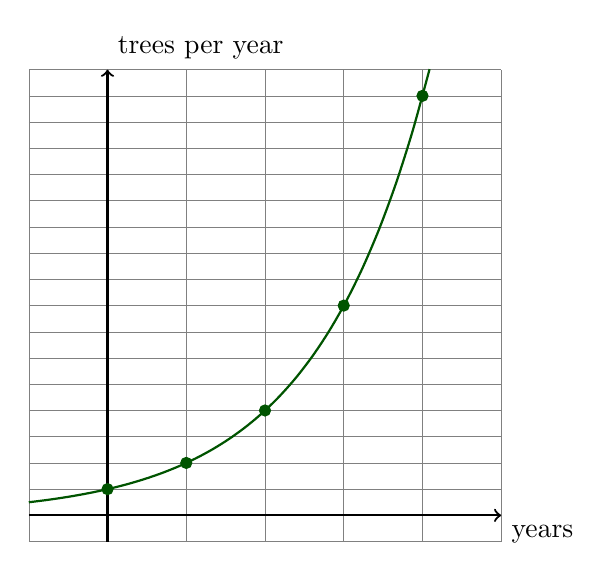
\begin{tikzpicture}
[
	closedpt/.style={circle,draw,fill,inner sep=0pt,minimum size=4pt},
	openpt/.style={circle,draw,inner sep=0pt,minimum size=4pt},
	yscale=0.333
]

	% grid
	\foreach \x in {\xmin,0,1,...,\xmax} {
		\draw[very thin,gray] (\x,\ymin) -- (\x,\ymax);
	}
	\foreach \y in {\ymin,0,1,...,\ymax} {
		\draw[very thin,gray] (\xmin,\y) -- (\xmax,\y);
	}

	% label grid
	% \foreach \x in {1,2,3,4} {
	% 	\node[below] at (\x,0) {$\x$};
	% }
	% \foreach \y in {0.5,1} {
	% 	\node[left] at (0,\y) {$\y$};
	% }

	% axes
	\draw[->,thick] (\xmin,0) -- (\xmax,0) node[below right] {years};
	\draw[->,thick] (0,\ymin) -- (0,\ymax) node[above right] {trees per year};

	\draw[green!33!black,smooth,domain=-1:4.09,thick] plot (\x, {exp (0.693 * \x)});

	% data
	\node[green!33!black,closedpt] at (0,1) {};
	\node[green!33!black,closedpt] at (1,2) {};
	\node[green!33!black,closedpt] at (2,4) {};
	\node[green!33!black,closedpt] at (3,8) {};
	\node[green!33!black,closedpt] at (4,16) {};

\end{tikzpicture}
